
\section{Learning to optimize with unrolled ISTA}
\parttitleframe{Moreau2017a,Ablin2019}


% \frame{
%     \frametitle{Solving many inverse problems}


%     \hskip-.7ex{\bf Context:} Many inverse problems with the same structure $G$.\\[1em]
%     \myitem{} One per time sample for MEG: $> 50k$ instances.\\[1em]
%     \begin{columns}[c]

%         \column{.55\textwidth}

%         {\bf Goal:} learn $\Phi_\Theta$ with $T$ layers such that:
%         \[
%             F_x(\Phi_\Theta(x)) \le F_x(ISTA_T(x))
%         \]
%         \strongpoint{Find the same solution as ISTA!}

%         \vskip1em

%         {\bf Questions:}\\[1em]
%         \myitem{} How fast can LISTA go?\\[.5em]
%         \myitem{} What does LISTA learn?\\[1em]

%         \column{.45\textwidth}
%         {\centering
%         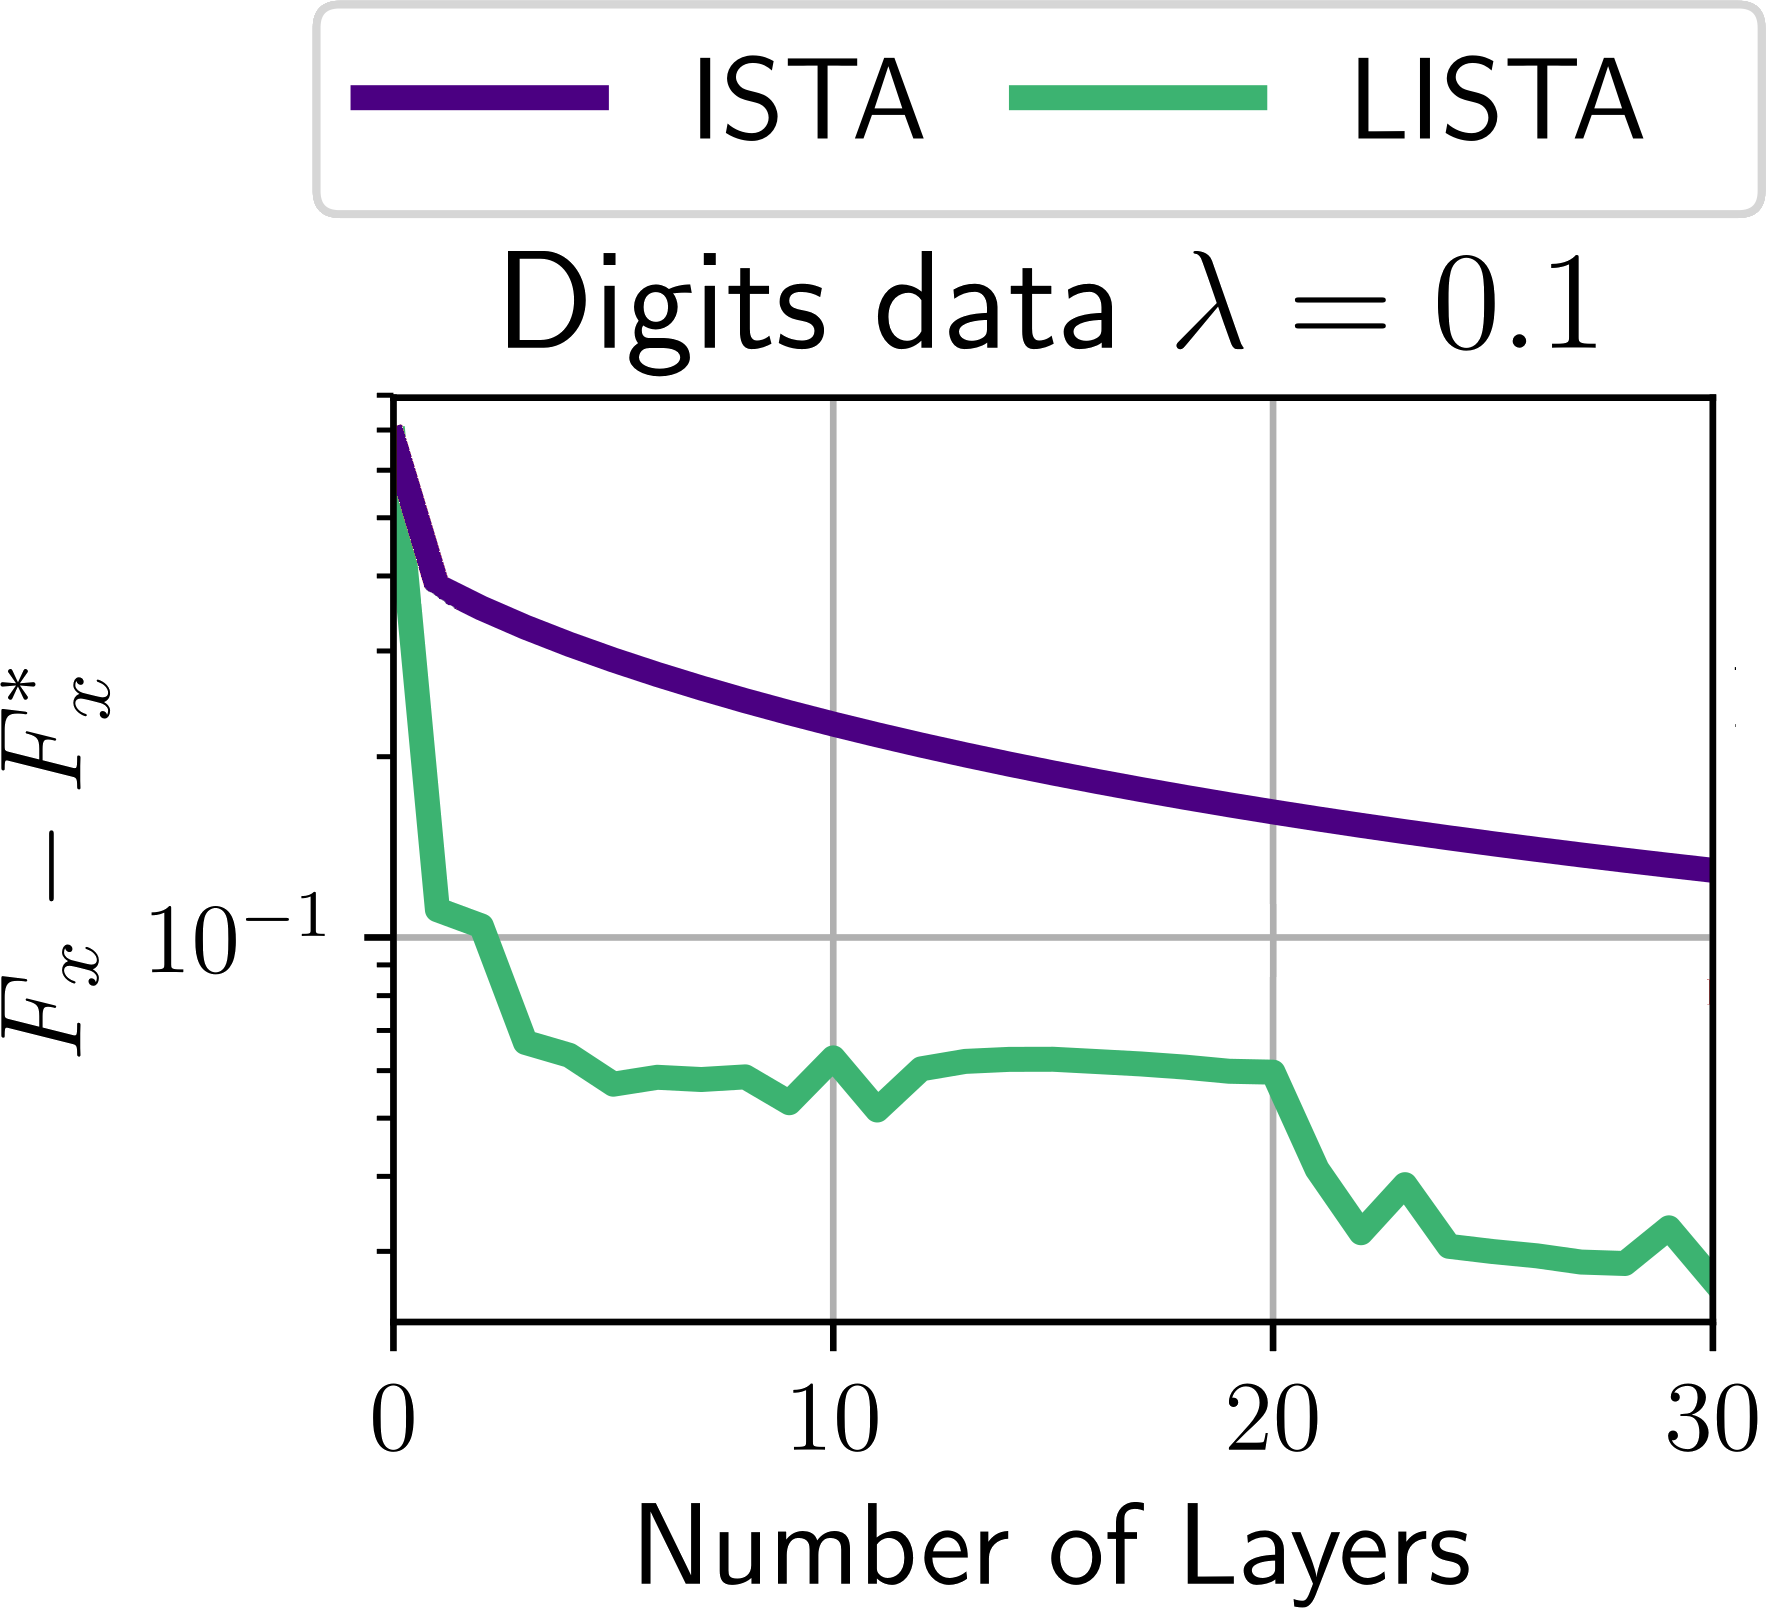
\includegraphics[width=\textwidth]{comparison_lista.png}\\}
%     \end{columns}
% }


\frame{
    \frametitle{How fast can LISTA go? \contrib{Moreau and Bruna, 2017}}

    Results are based on a quasi-diagonalization $G^\top G \simeq V^\top \Lambda V$ that does not distort ``too much'' the $\ell_1$-norm.\\[2em]

    \myitem{} For a class of parameters, LISTA has the same cvg rate as ISTA.\\[1em]
    \myitem{} LISTA can benefit from improved constants.\\[1em]
    \myitem{} As the optimization approaches a solution, it is harder and harder to get improved constants.\\[2em]


    \strongpoint{Shows that it is possible to improve the first iterations of the algorithm.}
}



\begin{frame}[t]{ISTA: Majoration-Minimization}
    Taylor expansion of $f_x$ in $z^{(t)}$
    \begin{align*}
        F_x(z) &  = f_x(z^{(t)}) + \nabla f_x(z^{(t)})^\top(z - z^{(t)})
                    + \frac{1}{2}\|G(z-z^{(t)})\|_2^2+ \lambda\|z\|_1\\
               & \le f_x(z^{(t)}) + \nabla f_x(z^{(t)})^\top(z - z^{(t)}) + \frac{L}{2}\|z - z^{(t)}\|_2^2 + \lambda\|z\|_1
    \end{align*}
    $\Rightarrow$ Replace the Hessian $G^\top G$ by an upper bound $L \textbf{ Id}$.\\[2em]

    \only<1>{
    Separable function that can be minimized in close form
    \begin{align*}
        \argmin_z \frac{L}{2}\left\|z^{(t)} - \frac{1}{L}\nabla f_x(z^{(t)}) - z\right\|_2^2 + \lambda\|z\|_1
        & = \text{prox}_{\frac{\lambda}{L}}\left(z^{(t)} - \frac{1}{L}\nabla f_x(z^{(t)})\right)\\
        & = \text{ST}\left(z^{(t)} - \frac{1}{L}\nabla f_x(z^{(t)}),
                           \frac{\lambda}{L}\right)
    \end{align*}
    }
    \only<2>{
        By design,
        \[
            F(z^{t+1}) \le Q^t(z^{t+1}) \le Q^t(z^{t+1}) = F(z^t)
        \]
        and the algorithm converges.\\[2em]
        The key is to find a majorant easy to minimize.
    }
\end{frame}


\begin{frame}{ISTA: Majoration for the data-fit}
    \definecolor{darkgreen}{RGB}{0, 148, 0}
    \myitem{} Level sets for $z^\top G^\top G z
                       \only<2>{\le \color{red} L \|z\|_2}
                       \only<3>{\le \color{blue} z^\top V^\top \Lambda V z}$
              \only<3>{\contrib{Moreau and Bruna, 2017}}\\
    \centering
    \makebox[.75\textwidth][c]{
        \only<1>{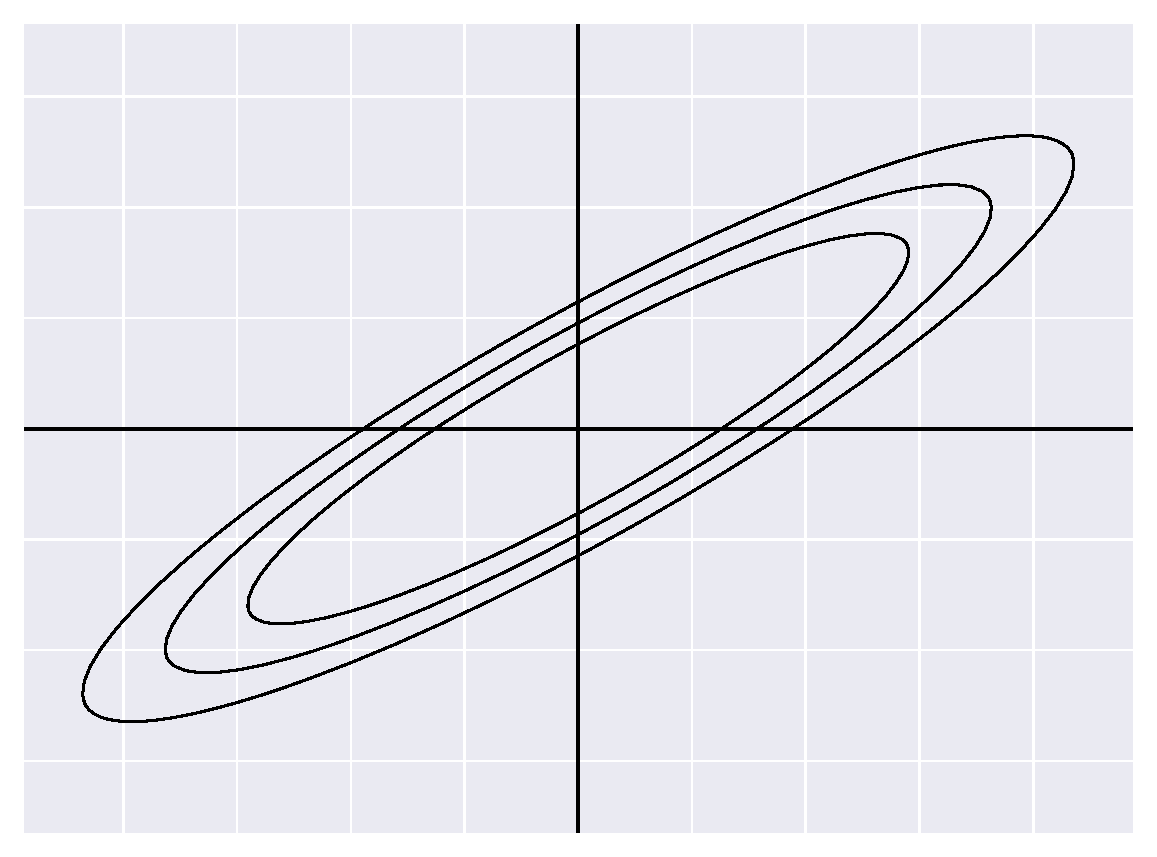
\includegraphics[height=.75\textheight]{ell1}}%
        \only<2>{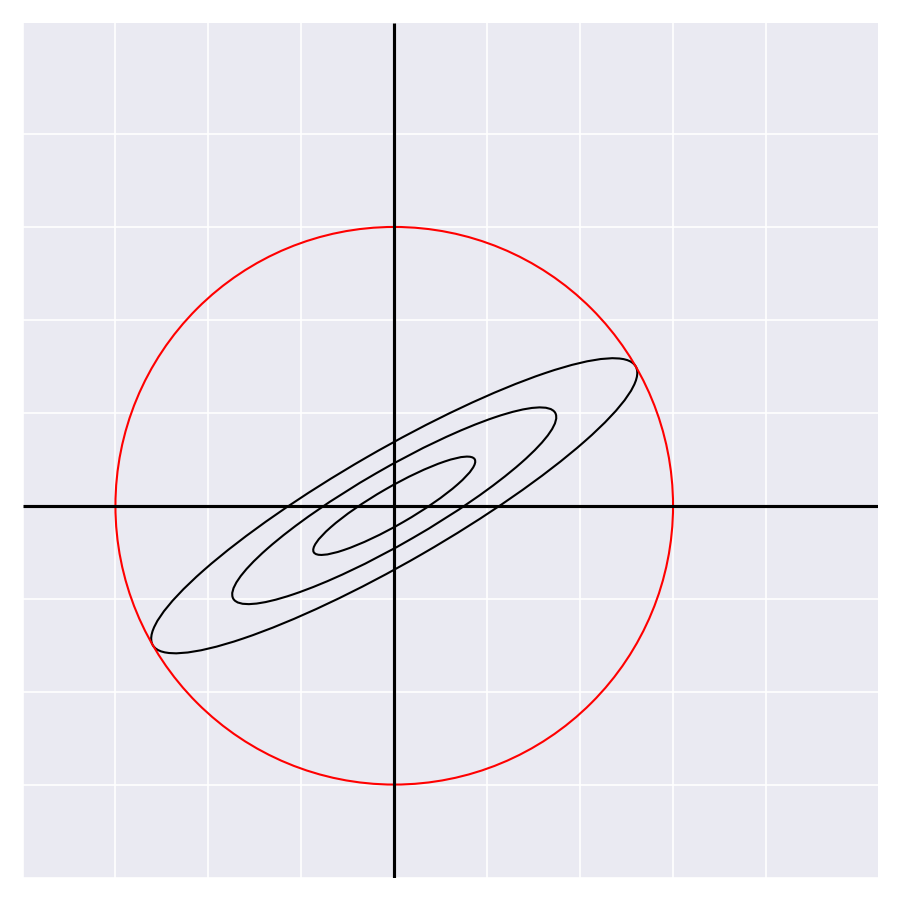
\includegraphics[height=.75\textheight]{ell2}}%
        \only<3>{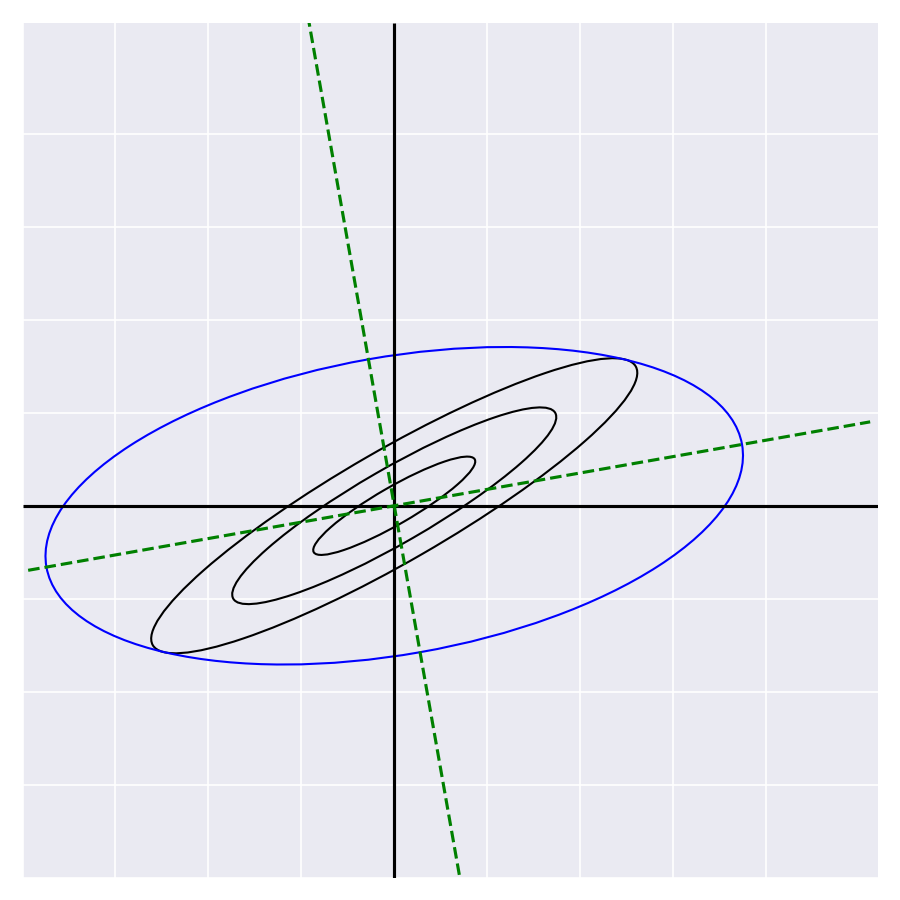
\includegraphics[height=.75\textheight]{ell3}}
    }\\
\end{frame}


\frame{
    \frametitle{What does LISTA learn? \contrib{Ablin et al., 2019}}

    Consider that the number of layers goes to $+\infty$.\\[1em]
    \begin{block}{Theorem -- Asymptotic convergence of the weights}
        Assume that the weights of the network converge to a limit:
        \[
            W_z^{(t)}, W_X^{(t)}, \beta^{(t)} \to W_z^*, W_X^*, \beta^*
            \qquad as \qquad t\to +\infty
        \]
        and that the output of the network converges to a solution of the unsupervised problem.\\[.5em]
        Then
        \[
            W_z^* = Id - \alpha D^\top D, \quad
            W_X^* = \alpha D^\top, \quad
            \beta^* = \alpha \lambda, \quad
        \]
    \end{block}

    \strongpoint{Correspond to ISTA with a learned step size $\alpha$}
}

% \frame{
%     \frametitle{Intuition for the result}

%     The network's output $\Phi(x)$ for all input $x$ needs to verify:
%     \begin{align*}
%         \Phi(x) = & ~ st\big(
%             \textcolor{linkcolor}{(Id - \frac1L G^\top G)}\Phi(x)
%             + \textcolor{D}{\frac1L G^\top} x,
%             \textcolor{Z}{\frac\lambda{L}}
%         \big) \qquad\qquad\keypoint{\text{KKT}}\\[.5em]
%         \Phi(x) = &~st\big(
%             \textcolor{linkcolor}{W_z^*}\Phi(x)
%             + \textcolor{D}{W_X^*} x,
%             \textcolor{Z}{\beta^*}
%         \big) \qquad\qquad\quad\keypoint{\text{Weights cvg}}
%     \end{align*}
%     \vskip2em
%     \myitem{} If verified uniformly, this imposes a strong structure on the asymptotic weights.\\[1em]
%     \myitem{} This structure can be relaxed based on the distribution of $x$.
% }

\begin{frame}{Numerical verification}
    \centering
    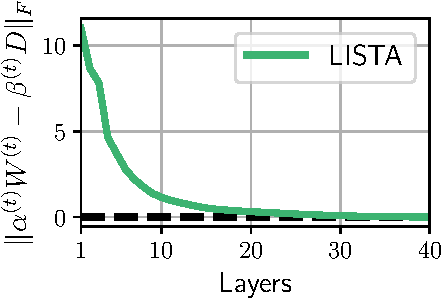
\includegraphics[width=.8\textwidth]{fro_similarity}\\[1em]
    40-layers LISTA network trained on a $10 \times 20$ problem with $\lambda = 0.1$\\
    {\bf The weights $W^{(t)}$ align with $D$ and $\alpha, \beta$ get coupled.}


\end{frame}


\begin{frame}{Step LISTA \contrib{Ablin et al., 2019}}

    Inspired by this result: learn adapted step sizes for ISTA.\\[2em]
    {\bf Restricted parametrization :}
    Only learn a step-size $\alpha^{(t)}$\\[1em]
    \[
    z^{(t+1)} = \text{ST}\left(z^{(t)}
              - \textcolor{linkcolor}{\bf\alpha^{(t)}} D^\top(D z^{(t)} -x),
              \lambda\textcolor{linkcolor}{\bf\alpha^{(t)}}\right)
    \]
    \vskip1em
    \underline{Fewer parameters:}\\[1em]
    % $T$ instead of $( 2 + mn)T~.$\\[1em]
    \begin{columns}[c]
        \column{.5\textwidth}
            \myitem{} Easier to learn\\
        \column{.5\textwidth}
            \myitem{} Fewer degrees of freedom\\
    \end{columns}
    \vskip2em
    \centering $\Rightarrow$ Reduced performances?\\

\end{frame}




\begin{frame}[t]{Performances}

    {\bf Simulated data:} $m=256$ and $n=64$\\[.7em]
    \hskip6ex $D_k \sim \mathcal U(\mathcal S^{n-1})$ and $x = \frac{\widetilde x}{\|D^\top \widetilde x\|_\infty}$ with $\widetilde x_i \sim \mathcal N(0, 1)$\\[1.5em]
    {\centering
    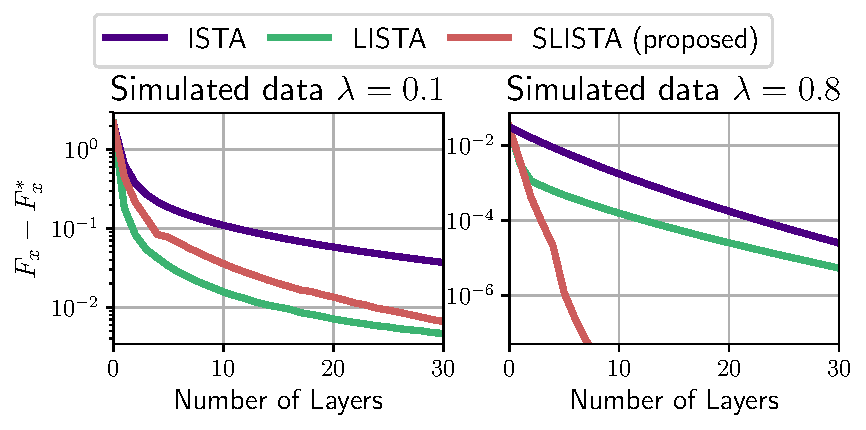
\includegraphics[width=\textwidth]{comparison_networks_simu}\\}
\end{frame}


\begin{frame}{Learning better step sizes}
    Linked to SLISTA when step sizes are in $\big[\frac1{L_S}, \frac2{L_S}\big[$ when $Supp(z^{(t)}) = S$\\[.5em]
    $L_S$ is the largest eigenvalue of $G^\top G$ restricted on the support $S$\[
        \max_{\substack{Supp(z) = S\\\|z\|_2\le 1}} z G^\top G z
    \]
    \centering
    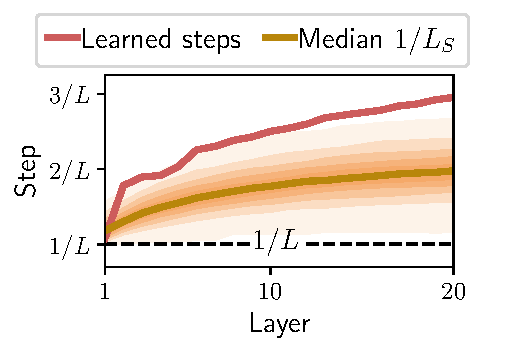
\includegraphics[width=.6\textwidth]{learned_steps}\\
    % The learned step-sizes are linked to the distribution of $1/L_S$\\[1em]


\end{frame}


\frame{
    \frametitle{Unrolling for learned optimization}

    \vskip4em
    {\centering\bf No hope to learn an algorithm that converges\\faster than ISTA \underline{uniformly}.\\[2em]}

    \begin{itemize}\itemsep.5em
        \item But one can learn parameters (step-size) of the algorithm that better adapt to the input distribution.\\
        \contrib{Ablin et al., 2019}
        \item Also possible to improve the first iterations of ISTA (improve constants).\\
        \contrib{Moreau and Bruna, 2017}
    \end{itemize}

    \vspace{0pt plus 1 filll}
    \footnotesize
    Also considered unrolled algorithms for TV in  Cherkaoui, Sulam, {\bf M.}, NeurIPS 2020.

}
